% Template for a Computer Science Tripos Part II project dissertation
\documentclass[12pt,a4paper,twoside,openright]{report}
\usepackage[pdfborder={0 0 0}]{hyperref}    % turns references into hyperlinks
\usepackage[margin=25mm]{geometry}  % adjusts page layout
% allows inclusion of PDF, PNG and JPG images
\usepackage{graphicx}
\usepackage{amsmath}
\usepackage{bbm} %Used for the indicator function
\graphicspath{ {figs/} }

\usepackage{verbatim}
\usepackage{docmute}   % only needed to allow inclusion of proposal.tex


\usepackage{listings} % Package to display code and customize highlighting
\usepackage{color}
 
\definecolor{codegreen}{rgb}{0,0.6,0}
\definecolor{codegray}{rgb}{0.5,0.5,0.5}
\definecolor{codepurple}{rgb}{0.58,0,0.82}
\definecolor{backcolour}{rgb}{0.95,0.95,0.92}
 
\lstdefinestyle{mystyle}{
    backgroundcolor=\color{backcolour},   
    commentstyle=\color{codegreen},
    keywordstyle=\color{magenta},
    numberstyle=\tiny\color{codegray},
    stringstyle=\color{codepurple},
    basicstyle=\footnotesize,
    breakatwhitespace=false,         
    breaklines=true,                 
    captionpos=b,                    
    keepspaces=true,                 
    numbers=left,                    
    numbersep=5pt,                  
    showspaces=false,                
    showstringspaces=false,
    showtabs=false,                  
    tabsize=2
}
\lstset{style=mystyle} % Set code listings style

\raggedbottom                           % try to avoid widows and orphans
\sloppy
\clubpenalty1000%
\widowpenalty1000%

\renewcommand{\baselinestretch}{1.1}    % adjust line spacing to make
                                        % more readable

\begin{document}

\bibliographystyle{plain}


%%%%%%%%%%%%%%%%%%%%%%%%%%%%%%%%%%%%%%%%%%%%%%%%%%%%%%%%%%%%%%%%%%%%%%%%
% Title


\pagestyle{empty}

\rightline{\LARGE \textbf{Sebastian Borgeaud dit Avocat}}

\vspace*{60mm}
\begin{center}
\Huge
\textbf{Brain tumour segmentation using Convolutional Neural Networks} \\[5mm]
Computer Science Tripos -- Part II \\[5mm]
Fitzwilliam College \\[5mm]
\today  % today's date
\end{center}

%%%%%%%%%%%%%%%%%%%%%%%%%%%%%%%%%%%%%%%%%%%%%%%%%%%%%%%%%%%%%%%%%%%%%%%%%%%%%%
% Proforma, table of contents and list of figures

\pagestyle{plain}

\chapter*{Proforma}

{\large
\begin{tabular}{ll}
Name:               & \bf Martin Richards                       \\
College:            & \bf St John's College                     \\
Project Title:      & \bf How to write a dissertation in \LaTeX \\
Examination:        & \bf Computer Science Tripos -- Part II, July 2001  \\
Word Count:         & \bf 1587\footnotemark[1]
                      (well less than the 12000 limit)  \\
Project Originator: & Dr M.~Richards                    \\
Supervisor:         & Dr Markus Kuhn                    \\ 
\end{tabular}
}
\footnotetext[1]{This word count was computed
by \texttt{detex diss.tex | tr -cd '0-9A-Za-z $\tt\backslash$n' | wc -w}
}
\stepcounter{footnote}


\section*{Original Aims of the Project}

To write a demonstration dissertation\footnote{A normal footnote without the
complication of being in a table.} using \LaTeX\ to save
student's time when writing their own dissertations. The dissertation
should illustrate how to use the more common \LaTeX\ constructs. It
should include pictures and diagrams to show how these can be
incorporated into the dissertation.  It should contain the entire
\LaTeX\ source of the dissertation and the makefile.  It should
explain how to construct an MSDOS disk of the dissertation in
Postscript format that can be used by the book shop for printing, and,
finally, it should have the prescribed layout and format of a diploma
dissertation.


\section*{Work Completed}

All that has been completed appears in this dissertation.

\section*{Special Difficulties}

Learning how to incorporate encapulated postscript into a \LaTeX\
document on both Ubuntu Linux and OS X.
 
\newpage
\section*{Declaration}

I, [Name] of [College], being a candidate for Part II of the Computer
Science Tripos [or the Diploma in Computer Science], hereby declare
that this dissertation and the work described in it are my own work,
unaided except as may be specified below, and that the dissertation
does not contain material that has already been used to any substantial
extent for a comparable purpose.

\bigskip
\leftline{Signed [signature]}

\medskip
\leftline{Date [date]}

\tableofcontents

\listoffigures

\newpage
\section*{Acknowledgements}

This document owes much to an earlier version written by Simon Moore
\cite{Moore95}.  His help, encouragement and advice was greatly 
appreciated.

%%%%%%%%%%%%%%%%%%%%%%%%%%%%%%%%%%%%%%%%%%%%%%%%%%%%%%%%%%%%%%%%%%%%%%%
% now for the chapters

\pagestyle{headings}

\chapter{Introduction [14\%]}
Convolutional Neural Networks have gained an enormous amount of traction in recent years, as they have been used in many different areas to obtain state-of-the-art results. The areas of computer vision and biomedical imaging analysis are no exception to this and the number of entries using Convolutional Neural Networks in the BraTS [CITATION] challenge has risen accordingly, with some of these entries being at the top of the evaluation board.

\chapter{Preparation [26\%]}
During the first phase of my project, the aim was to replicate the method used by Pereira et al \cite{pereira}, so it was crucial to first fully understand the steps taken in the paper to then be able to reimplement them. Unfortunately, the paper didn't include any source code which meant that if something wasn't fully explained in details, I would have to find out what was actually done. This turned out to be a problem for the pre-processing step as the proposed method uses a normalisation developed by Nyul [CITATION]. This normalisation requires human input, preferably from a domain expert, and I was therefore not able to use that normalisation method. The paper also proposed a second normalisation method, which used a combination of winsorizing and N4 normalization. This method performed slightly worse but had the advantage of being fully automated, which is why I chose to use this method.\\

\section{Convolutional Neural Networks}
\subsubsection{Neural networks}
To understand how convolutional neural networks work, it is important to be familiar with ordinary neural networks. These are made up of layers of neurons that have trainable weights in a sequence of layers. An example of the structure of such a neural network can be found in figure \ref{fig:nn_layout}.
\begin{figure}
	\centering
	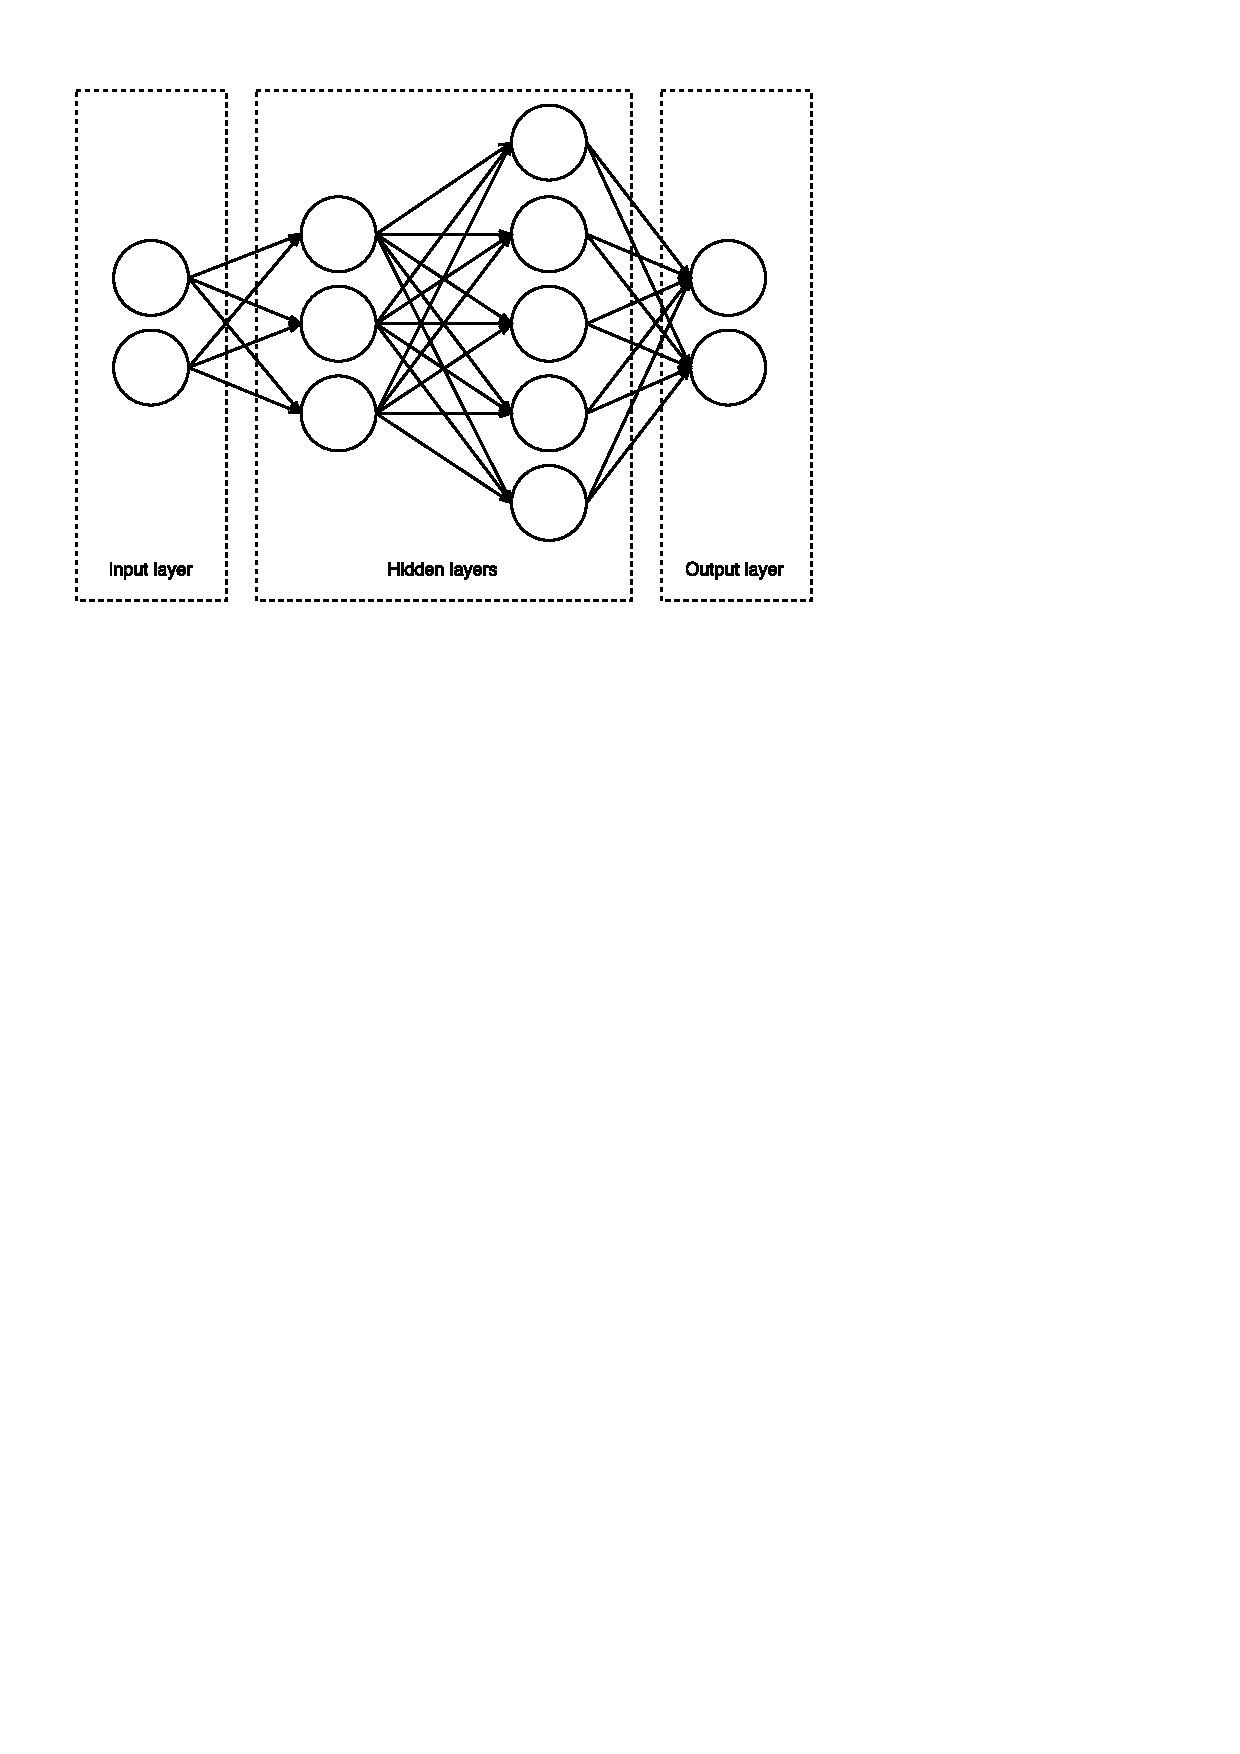
\includegraphics[scale=0.6]{nn_layout}
	\caption{Structure of a simple neural network with two hidden layers.}
	\label{fig:nn_layout}
\end{figure}

Each neuron in layer $n+1$ is connected to every neuron in layer $n$ and computes as an output
\[y = f_{act}((\sum_{i=1}^{n} y_i w_i) + b)\]
where $f_{act}$ is a non-linear, differentiable activation function and $y_i$ is the output of neuron $i$ in the previous layer. A neuron is connected to every neuron in the previous layer, which is why this layer is also referred to as a fully connected layer.
\subsubsection{Activation functions}
The most common activation functions are the Sigmoid function,
\[S(x) = \frac{1}{1 + e^x}\] the hyperbolic tangent 
\[\textrm{tanh}(x)=\frac{e^x - e^{-x}}{e^x + e^{-x}}\] the rectifier 
\[
f(x) = 
\begin{cases}
	0 & \text{if } x < 0\\
	x & \text{otherwise}
\end{cases}
\]
and the leaky rectifier, for some $0 < \alpha < 1$
\[
f(x) = 
\begin{cases}
	\alpha x & \text{if } x < 0\\
	x & \text{otherwise}
\end{cases}
\]
This functions can be seen in figure \ref{fig:activation_functions}
\begin{figure}
	\centering
	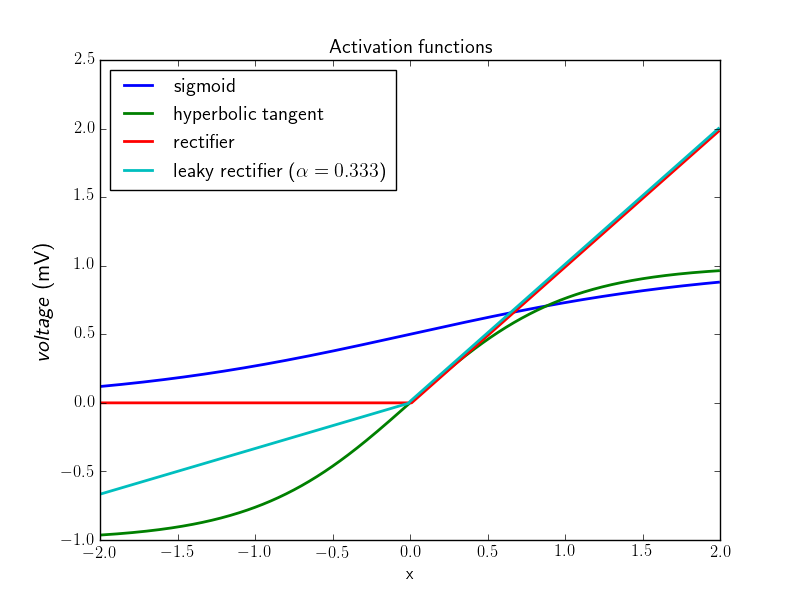
\includegraphics[scale=0.6]{activations}
	\caption{Plot of 4 different activation functions.}
	\label{fig:activation_functions}
\end{figure}
Historically the hyperbolic tangent function or the sigmoid function have been used as activation functions. However, as the magnitude of the gradients of those functions is always below 1, these activation function create a problem of vanishing gradients for deeper networks, as we have to multiply those gradients together for each layer. [CITATIONS!!!!] This is why it is now preferred to use the rectifier or the leaky rectifier functions.
[PLOT OF FUNCTIONS]
\subsubsection{Loss function}
The next step is to compute how well our network approximates our training data with a loss function, to then decide how to change the weights of the network in order to minimise the loss. Since the aim of the network is to classify the central pixel(s) of the patch, we use the categorical cross-entropy loss function
\begin{equation}
	\mathcal{L}(\theta) = 
	\frac{1}{m}\Big[\sum_{i=1}^m \sum_{j=1}^k\mathbbm{1}[y^{(i)} = k]\log(P(y^{(i)}=k \mid x^{(i)};\theta))\Big]
\end{equation}
where $\mathbbm{1}$ is the indicator function, $\log(P(y^{(i)}=k \mid x^{(i)};\theta))$ is the probability outputted by the network.
\subsubsection{Backpropagation}
Since every basic operation used in the neural network is differentiable, the entire network will also be differentiable, which in turn makes it possible to calculate the gradient of a loss function with respect to the weights in the network. This then will allow us to minimise this loss function by using a gradient descent approach.

\subsubsection{SGD}

\subsubsection{Momentum}
\subsubsection{Further optimizations}
\subsection{Adding convolutions}
Convolutional neural networks are similar to ordinary neural networks, sometimes also called artificial neural networks. Convolutional neural networks are also made up for neurons that have trainable weights. The main difference is that
\subsection{Dropout}
\subsection{Batch Normalization}

\section{Data pre-processing}
\subsection{N4ITK}
\subsection{Patch extraction}

\section{Data source}

\chapter{Implementation [40\%]}
\section{CNN models}
I implemented the convolutional neural networks using the Keras (Add reference) library, which allows users to create neural networks by combining different layers together. The more common layers come as part of the library but Keras allows the user to define layers as well.  The architecture proposed by Pereira et al \cite{pereira} used the following layers:
\begin{itemize}
	\item two-dimensional convolutional layers
	\item fully connected layers
	\item two-dimensional max pooling layers
\end{itemize}
Futhermore, we can easily add Dropout to the model by adding an instance of a Dropout layer where required. 

My implementation of the model proposed by Pereira \cite{pereira} looks as follows in Keras:
\lstinputlisting[language=Python, firstline=24, lastline=60]{../Work/model.py}

This makes it easy to create deep, convolutional networks and to experiment with them. This reason, together with the active community of Keras users is why I chose to use the Keras library.

Before training the models, we further need to specify which loss function and which algorithm should be used to respectively specify and minimise the loss function. Again, keras makes this very simple:
\lstinputlisting[language=Python, firstline=71, lastline=72]{../Work/model.py}

\section{Data preprocessing}

\section{Training}

\section{Segmentation}

\chapter{Evaluation + Conclusion [20\%]}

\section{Metrics used for the evaluation}
\subsection{Dice score}
\subsection{Positive predictive value}
\subsection{Sensitivity}

\section{Evaluation of the model proposed by Pereira et al.}
\section{Evaluation of the my model}
\section{Comparison}

\chapter{Conclusion}

I hope that this rough guide to writing a dissertation is \LaTeX\ has
been helpful and saved you time.


%%%%%%%%%%%%%%%%%%%%%%%%%%%%%%%%%%%%%%%%%%%%%%%%%%%%%%%%%%%%%%%%%%%%%
% the bibliography
\addcontentsline{toc}{chapter}{Bibliography}
\bibliography{refs}

%%%%%%%%%%%%%%%%%%%%%%%%%%%%%%%%%%%%%%%%%%%%%%%%%%%%%%%%%%%%%%%%%%%%%
% the appendices
%\appendix
%
%\chapter{Latex source}
%
%\section{diss.tex}
%{\scriptsize\verbatiminput{diss.tex}}
%
%%\section{proposal.tex}
%{\scriptsize\verbatiminput{proposal.tex}}
%
%\chapter{Makefile}
%
%\section{makefile}\label{makefile}
%{\scriptsize\verbatiminput{makefile.txt}}
%
%\section{refs.bib}
%{\scriptsize\verbatiminput{refs.bib}}
%
%
%\chapter{Project Proposal}
%
%%% Note: this file can be compiled on its own, but is also included by
% diss.tex (using the docmute.sty package to ignore the preamble)
\documentclass[12pt,a4paper,twoside]{article}
\usepackage[pdfborder={0 0 0}]{hyperref}
\usepackage[margin=25mm]{geometry}
\usepackage{graphicx}
\usepackage{parskip}
\begin{document}

\begin{center}
\Large
Computer Science Tripos -- Part II -- Project Proposal\\[4mm]
\LARGE
Brain tumour segmentation using Convolutional Neural Networks

\large
S.~Borgeaud~dit~Avocat, Fitzwilliam College

Originator: D.~Wang

11 October 2016
\end{center}

\vspace{5mm}

\textbf{Project Supervisor:} Dr M.~Jamnik \& D.~Wang

\textbf{Director of Studies:} Dr R.~K.~Harle

\textbf{Project Overseers:} Prof J.~Bacon  \& Prof R.~Anderson

% Main document

\section*{Introduction}

Over the last years deep learning, more specifically convolutional neural networks (CNN), have outperformed other machine learning techniques in many tasks such as image classification \cite{nature-deep-learning-review}. The field of bioinformatics is no exception to this, in particular, convolutional neural networks have been shown to perform as well as previous state-of-the-art algorithms on the problem of brain tumour segmentation \cite{brats-proceedings}.

The aim of this project is to use convolutional neural networks to replicate these recent results on the brain tumour segmentation problem. This project will concentrate exclusively on the dataset provided by the BraTS2013\footnote{\url{http://martinos.org/qtim/miccai2013/}} grand challenge on which many different algorithms have already been tested and will provide a good framework to test and compare my work.

As a starting point I will follow the paper written by Pereira et al \cite{pereira}. The approach used is to cut the magnetic resonance images into multiple patches and regard the problem as a classification problem of the pixel located at the center of the patch. The aim is to classify each pixel into one of these four classes:
\begin{enumerate}
	\item Non-tumor
	\item Surrounding edema
	\item Non-enhancing tumour
	\item Enhancing tumour
\end{enumerate}
\section*{Starting point}
  
The starting point for this project is the part 1B course 'Artificial Intelligence 1'  which provided a short introduction to machine learning. In particular multi-layer perceptrons, the sigmoid activation function, backpropagation and stochastic gradient descent training were introduced. These concepts are all reused in convolutional neural networks which add convolutional and pooling layers to conventional multi-layer perceptrons network.

I will be using the Keras library with Tensor Flow to create and train convolutional neural networks.

Keras is a library written for Python. Fortunately, I have used Python before in small side projects meaning that I won't have to spend time learning a new language.

As the problem is self contained and formulated purely as a a machine learning task, none or very little biological/medical background knowledge is required.

\section*{Resources required}

For this project I will mainly use my own quad-core computer which
runs Mac OS X El Capitan. I accept full responsibility for this machine and I have made contingency plans to protect myself against hardware and/or software failure. In case of failure, I will be able to terminate my project using the MCS machines.  Backups will be to my external hard disk. Once a week, I will also copy all files to my Google Drive to add an extra level of redundancy in case of hardware failure. All written code will be under version control using git and will be backed up on a private GitHub repository at least daily while working on it. 

I will also need a computer with an external GPU to train the neural network in a reasonable amount of time. For this, I will be using the Cambridge High Performance cluster. Alternatively, if this is not possible, I will use a GPU that would be provided by the AI group.

\section*{Work to be done}

The project breaks down into the following phases:

\begin{enumerate}

\item The first phase of the project will be mainly focused on research during which I will learn how convolutional networks  work and read up on how they have been used on the brain tumour segmentation problem in different papers. I plan to complete the Stanford CS321n\footnote{\url{http://cs231n.github.io/}} course on convolutional neural networks that I have already started. I will also need to learn how to use the Keras and TensorFlow libraries and review some of the more advanced Python features that I haven't used recently.

\item The second phase will mainly be devoted to preparing the images obtained from the BRATS dataset. The images will need to be cut into patches each of which will have to be normalised. I will need to perform bias field correction as magnetic resonance images can exhibit non-uniformities that are the result of magnetic field variations rather than anatomical differences \footnote{\url{http://brainsuite.org/processing/surfaceextraction/bfc/}}. I will then need to perform intensity normalisation across the different images. Finally, I will need to add the correct label to each patch using the segmentation provided with the original training images.

\item The next step will be to use the prepared and normalised patches to train a convolutional neural network using the Keras library. This will require hyperparameter tuning using cross-validation to avoid overfitting. I will then construct segmented images using my convolutional neural network to delimit the different segments to get a visual result that is easy to interpret.

\item During the last step I will evaluate how well my convolutional neural network performed using standard methods used to evaluate classifiers such as the confusion matrix, recall, precision and Dice scores. This evaluation can be done for different hyperparameters. Because the dataset has been used many times before as part of the Grand Challenge\footnote{\url{https://grand-challenge.org}} I will also be able to perform a quantitative comparison with different segmentation algorithms also using convolutional neural networks as well as other algorithms using different techniques.

\end{enumerate}

\section*{Success criteria}

The main success criteria for this project will be to have an algorithm that performs brain tumour segmentation into the 4 different segments as discussed earlier. 

The primary aim is to achieve similar results to those obtained by Pereira et al \cite{pereira}, hopefully achieving 90\% of the accuracies obtained in the paper. This means achieving the Dice\footnote{\url{https://en.wikipedia.org/wiki/Sorensen-Dice\_coefficient}} scores summarised in the following table, where `complete' refers to the complete tumour region (including classes 2--4), `core' refers to all regions except for the edema structure (classes 3--4) and `enhancing' includes only the enhancing tumour (class 4):

\begin{center}
\begin{tabular}{ |c|c|c| } 
\hline
complete & core & enhancing \\
\hline
 0.79 & 0.74 & 0.69  \\ 
\hline
\end{tabular}
\end{center}



\section*{Possible extensions}

Due to the recent development of this area, this project naturally leads to multiple possible extensions:
\begin{enumerate}
	\item This process of segmenting MRI scans is very slow as each scan has to be cut into patches, one per pixel, and each patch then needs to be classified. Recent techniques have shown that it is possible to classify all pixels of a patch at once, which would drastically improve the speed of the segmentation. A possible extension would be to try to improve the segmentation speed using the suggested technique. It would then be interesting to compare the performance of the faster algorithm to the performance of the original one.
	\item Experiment with the layout of the neural network, in particular change the number of layers and the type of the layers of the convolutional neural network to try to improve the accuracy.
	\item Instead of using the Keras library, implement similar functionality myself using TensorFlow. I could then compare the results obtained by my implemention with those obtained using Keras. This will show and require a deeper understanding of how convolutional neural networks work.
	\item Use different data prepocessing/normalisation techniques and analyse how they affect the final accuracy of the convolutional neural network.
	\item Apply more recent techniques used to improve convolutional neural networks such as Dropout \cite{dropout}, Maxout \cite{maxout} or Batch Normalization \cite{batch_normalization} in order to improve the accuracy of the classification.
\end{enumerate}

\section*{Timetable}

Planned starting date is 21/10/2016.

\subsection*{Michaelmas term}
\begin{enumerate}
\item \textbf{Weeks 3--4} Learn about Convolutional Neural Networks by finishing the CS321n online course. Read papers about using Convolutional Neural Networks for brain tumour segmentation.

\emph{Milestone:} Understand the theory behind convolutional neural networks and be familiar with some of the more recent applications of them on the brain tumour segmentation problem.

\item \textbf{Weeks 5--6} Become familiar with the Keras library and refresh my Python knowledge. Download and play with the dataset.

\emph{Milestone:} Be comfortable enough with Keras and Python to be able to start the main part of the project.

\item \textbf{Weeks 7--8} Prepare the dataset for the implementation of the convolutional neural network. This includes performing the different normalisations.

{Milestone:} Have the dataset ready, that is split up into normalised patches. Each patch should have the corresponding label for the pixel that is located at its center.

\item \textbf{Christmas Vacation} Implement and train a convolutional neural network and perform the necessary cross-validation on the different hyperparameters. Create segmented brain images using my classifier.

{Milestone:} Have a working convolutional neural network that is able to classify the different patches with the required accuracy mentioned in the primary success criteria. Have some images that are segmented using the trained classifier.
\end{enumerate}


\subsection*{Lent term}
\begin{enumerate}

\item \textbf{Weeks 1--3} Write the progress report and prepare the presentation.

{Milestone:} Have the progress report submitted on time and be ready to give the presentation.

\item \textbf{Weeks 4--5} Evaluate the performance of my segmentation algorithm and look for possible improvements.

{Milestone:} Have the evaluation data of my convolutional neural network.

\item \textbf{Weeks 6--8} Compare the performance of my algorithm with the benchmarks available online and implement some of the extensions if time permits.

{Milestone:} Have all the necessary data for the final evaluation of my project.

\item \textbf{Easter Vacation} Write the main chapters of the dissertation. Implement some of the extensions if time permits.

{Milestone:} Have a complete first draft of my dissertation

\end{enumerate}

\subsection*{Easter term}
\begin{enumerate}
\item \textbf{Weeks 1--2} Improve the dissertation where necessary

{Milestone:} Have the dissertation in its final form
\item \textbf{Weeks 3--4} Proof read the dissertation and submit it.

{Milestone:} Have the dissertation submitted.

\end{enumerate}

\end{document}

\end{document}
